\documentclass[12pt]{article}

% report, book

%  Русский язык

\usepackage[T2A]{fontenc}
\usepackage[utf8]{inputenc}
\usepackage[english,russian]{babel}

\usepackage{amsmath,amsfonts,amssymb,amsthm,mathtools} 

\usepackage{graphicx}
\usepackage{listings}
\usepackage[table,xcdraw]{xcolor}

\usepackage{wasysym}

\usepackage{geometry} 
\geometry{a4paper,top=2cm,bottom=3cm,left=2cm}

\begin{document}

\begin{titlepage}
   \begin{center}
       \vspace*{1cm}

       \textbf{Лабораторная работа №1}

       \vspace{0.5cm}
        Алгоритмы одномерной минимизации функции
            
       \vspace{1.5cm}

       \textbf{Сысоев Александр, Зырянова Мария}
       
       \textbf{Верблюжий случай}

       \vfill
            
   \end{center}
\end{titlepage}

%1. Отчет должен содержать титульный лист, постановку задания, график
%исследуемой функции, аналитический вид решения (аналитическое значение
%координаты минимума вычислить с точностью до 4 значащих цифр).

%2. Отчет должен содержать таблицы с результатами исследований по каждому
%методу, где должны быть исходный и последующие интервалы, соотношение
%их длин, вычисляемые на них точки и значения функций.

%3. Необходимо построить график зависимости количества вычислений
%минимизируемой функции от логарифма задаваемой точности ε. Провести
%сравнение методов друг с другом. Отразить в отчете.

%4. По результатам численных вычислений сделать выводы, описать в отчете.

%5. Протестировать реализованные алгоритмы для задач минимизации
%многомодальных функций, например, на различных полиномах. Сделать
%выводы, описать в отчете.

\section{Постановка задания}

Необходимо реализовать алгоритмы одномерной минимизации функции:

\begin{itemize}
\item метод дихотомии
\item метод золотого сечения
\item метод Фиббоначи
\item метод парабол
\item комбинированный метод Брента
\end{itemize}

\section{Исследуемая функция}

Необходимо на интервале $[0.1; 2.5]$ найти минимум функции 

\begin{equation*}
f(x)=10xln(x)-\frac{x^2}{2}
\end{equation*}

$x_0$ -- точка локального экстремума $f(x)$, если $f'(x_0) = 0$:

\begin{equation*}
f'(x)=10+10ln(x)-x=0
\end{equation*}

\begin{figure}[h]
\centering
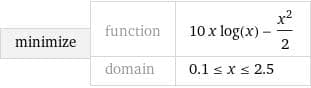
\includegraphics[width=0.5\textwidth]{problem.jpeg}
\caption{Нахождение локального минимума при помощи WolframAlpha}
\end{figure}

\begin{figure}[h]
\centering
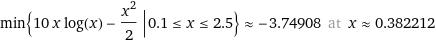
\includegraphics[width=0.5\textwidth]{solution.jpeg}
\caption{Найденное решение}
\end{figure}

\begin{figure}[h]
\centering
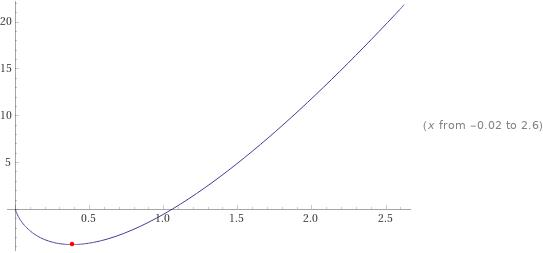
\includegraphics[width=0.5\textwidth]{graphic.jpeg}
\caption{График функции на исследуемом промежутке}
\end{figure}

\newpage
\section{Метод дихотомии}

Исследование проводится при $\epsilon = 0.0001$.

\begin{table}[h]
\begin{tabular}{|c|c|c|c|c|c|}
\hline
\rowcolor[HTML]{FFF0DB} 
\textbf{\begin{tabular}[c]{@{}c@{}}Левая \\ граница\end{tabular}} &
  \textbf{\begin{tabular}[c]{@{}c@{}}Правая \\ граница\end{tabular}} &
  \textbf{Отношение} &
  \textbf{Точка} &
  \textbf{\begin{tabular}[c]{@{}c@{}}Значение с\\ левой стороны\end{tabular}} &
  \textbf{\begin{tabular}[c]{@{}c@{}}Значение с \\ правой стороны\end{tabular}} \\ \hline
0.1     & 2.5     & --       & 1.3     & 2.56517  & 2.5663   \\ \hline
0.1     & 1.3     & 2        & 0.7     & -2.74201 & -2.74144 \\ \hline
0.1     & 0.7     & 2        & 0.4     & -3.74518 & -3.74514 \\ \hline
0.1     & 0.4     & 2        & 0.25    & -3.49678 & -3.49719 \\ \hline
0.25    & 0.4     & 2        & 0.325   & -3.70551 & -3.70566 \\ \hline
0.325   & 0.4     & 2        & 0.3625  & -3.74408 & -3.74413 \\ \hline
0.3625  & 0.4     & 2        & 0.38125 & -3.74907 & -3.74907 \\ \hline
0.38125 & 0.4     & 2        & 0.39062 & -3.74821 & -3.74819 \\ \hline
0.38125 & 0.39062 & 2.001067 & 0.38594 & -3.74891 & -3.7489  \\ \hline
0.38125 & 0.38594 & 1.997868 & 0.38359 & -3.74906 & -3.74906 \\ \hline
0.38125 & 0.38359 & 2.004274 & 0.38242 & -3.74908 & -3.74908 \\ \hline
0.38125 & 0.38242 & 2        & 0.38184 & -3.74908 & -3.74908 \\ \hline
0.38184 & 0.38242 & 2.017241 & 0.38213 & -3.74908 & -3.74908 \\ \hline
0.38213 & 0.38242 & 2        & 0.38228 & -3.74908 & -3.74908 \\ \hline
0.38213 & 0.38228 & 1.933333 & 0.3822  & -3.74908 & -3.74908 \\ \hline
\end{tabular}
\end{table}

Метод дихотомии показал, что функция на данном промежутке достигает минимума при значении $x_{min} = 0.3822021484375$, $f_{min} = -3.7490810073197856$. Выполнено 15 итераций.

\newpage
\section{Метод золотого сечения}

Исследование проводится при $\epsilon = 0.0001$.

\begin{table}[h]
\begin{tabular}{|c|c|c|c|c|c|c|}
\hline
\rowcolor[HTML]{FFF0DB} 
\textbf{\begin{tabular}[c]{@{}c@{}}Левая\\ граница\end{tabular}} &
  \textbf{\begin{tabular}[c]{@{}c@{}}Правая\\ граница\end{tabular}} &
  \textbf{Отношение} &
  \textbf{\begin{tabular}[c]{@{}c@{}}Левая\\ точка\end{tabular}} &
  \textbf{\begin{tabular}[c]{@{}c@{}}Значение в\\ левой точке\end{tabular}} &
  \textbf{\begin{tabular}[c]{@{}c@{}}Правая\\ точка\end{tabular}} &
  \textbf{\begin{tabular}[c]{@{}c@{}}Значение в\\ правой точке\end{tabular}} \\ \hline
0.1     & 2.5     & --       & 1.01672 & -0.34828 & 1.58328 & 6.02178  \\ \hline
0.1     & 1.58328 & 1.618036 & 0.66656 & -2.92587 & --      & --       \\ \hline
0.1     & 1.01672 & 1.618029 & 0.45016 & -3.69429 & --      & --       \\ \hline
0.1     & 0.66656 & 1.618046 & 0.31641 & -3.69104 & --      & --       \\ \hline
0.31641 & 0.66656 & 1.618049 & --      & --       & 0.53282 & -3.49645 \\ \hline
0.31641 & 0.53282 & 1.617994 & 0.39907 & -3.74556 & --      & --       \\ \hline
0.31641 & 0.45016 & 1.618019 & 0.36749 & -3.74632 & --      & --       \\ \hline
0.31641 & 0.39907 & 1.618074 & 0.34798 & -3.73386 & --      & --       \\ \hline
0.34798 & 0.39907 & 1.617929 & --      & --       & 0.37955 & -3.74899 \\ \hline
0.36749 & 0.39907 & 1.617796 & --      & --       & 0.38701 & -3.74879 \\ \hline
0.36749 & 0.38701 & 1.617828 & 0.37495 & -3.74841 & --      & --       \\ \hline
0.37495 & 0.38701 & 1.618574 & --      & --       & 0.3824  & -3.74908 \\ \hline
0.37955 & 0.38701 & 1.616622 & --      & --       & 0.38416 & -3.74903 \\ \hline
0.37955 & 0.38416 & 1.618221 & 0.38131 & -3.74907 & --      & --       \\ \hline
0.38131 & 0.38416 & 1.617544 & --      & --       & 0.38307 & -3.74907 \\ \hline
0.38131 & 0.38307 & 1.619318 & 0.38199 & -3.74908 & --      & --       \\ \hline
0.38199 & 0.38307 & 1.62963  & --      & --       & 0.38266 & -3.74908 \\ \hline
0.38199 & 0.38266 & 1.61194  & 0.38224 & -3.74908 & --      & --       \\ \hline
0.38199 & 0.3824  & 1.634146 & 0.38215 & -3.74908 & --      & --       \\ \hline
0.38215 & 0.3824  & 1.64     & --      & --       & 0.3823  & -3.74908 \\ \hline
0.38215 & 0.3823  & 1.666667 & 0.38221 & -3.74908 & --      & --       \\ \hline
\end{tabular}
\end{table}

Метод золотого сечения показал, что функция на данном промежутке достигает минимума при значении $x_{min} = 0.382224424485476$, $f_{min} = -3.7490810068327103$. Выполнена 21 итерация.

\newpage
\section{Метод Фибоначчи}

\begin{table}[h]
\begin{tabular}{|c|c|c|c|c|c|c|}
\hline
\rowcolor[HTML]{FFF0DB} 
\textbf{\begin{tabular}[c]{@{}c@{}}Левая \\ граница\end{tabular}} &
  \textbf{\begin{tabular}[c]{@{}c@{}}Правая \\ граница\end{tabular}} &
  \textbf{Отношение} &
  \textbf{\begin{tabular}[c]{@{}c@{}}Левая \\ точка\end{tabular}} &
  \textbf{\begin{tabular}[c]{@{}c@{}}Значение в \\ левой точке\end{tabular}} &
  \textbf{\begin{tabular}[c]{@{}c@{}}Правая \\ точка\end{tabular}} &
  \textbf{\begin{tabular}[c]{@{}c@{}}Значение в \\ правой точке\end{tabular}} \\ \hline
0.1     & 2.5     & --       & 1.01672 & -0.34828 & 1.58328 & 6.02178  \\ \hline
0.1     & 1.58328 & 1.618036 & 0.66656 & -2.92587 & --      & --       \\ \hline
0.1     & 1.01672 & 1.618029 & 0.45016 & -3.69429 & --      & --       \\ \hline
0.1     & 0.66656 & 1.618046 & 0.31641 & -3.69104 & --      & --       \\ \hline
0.31641 & 0.66656 & 1.618049 & --      & --       & 0.53282 & -3.49645 \\ \hline
0.31641 & 0.53282 & 1.617994 & 0.39907 & -3.74556 & --      & --       \\ \hline
0.31641 & 0.45016 & 1.618019 & 0.36749 & -3.74632 & --      & --       \\ \hline
0.31641 & 0.39907 & 1.618074 & 0.34798 & -3.73386 & --      & --       \\ \hline
0.34798 & 0.39907 & 1.617929 & --      & --       & 0.37955 & -3.74899 \\ \hline
0.36749 & 0.39907 & 1.617796 & --      & --       & 0.38701 & -3.74879 \\ \hline
0.36749 & 0.38701 & 1.617828 & 0.37495 & -3.74841 & --      & --       \\ \hline
0.37495 & 0.38701 & 1.618574 & --      & --       & 0.3824  & -3.74908 \\ \hline
0.37955 & 0.38701 & 1.616622 & --      & --       & 0.38416 & -3.74903 \\ \hline
0.37955 & 0.38416 & 1.618221 & 0.38131 & -3.74907 & --      & --       \\ \hline
0.38131 & 0.38416 & 1.617544 & --      & --       & 0.38307 & -3.74907 \\ \hline
0.38131 & 0.38307 & 1.619318 & 0.38199 & -3.74908 & --      & --       \\ \hline
0.38199 & 0.38307 & 1.62963  & --      & --       & 0.38266 & -3.74908 \\ \hline
0.38199 & 0.38266 & 1.61194  & 0.38224 & -3.74908 & --      & --       \\ \hline
0.38199 & 0.3824  & 1.634146 & 0.38215 & -3.74908 & --      & --       \\ \hline
0.38215 & 0.3824  & 1.64     & --      & --       & 0.38231 & -3.74908 \\ \hline
0.38215 & 0.38231 & 1.5625   & 0.38221 & -3.74908 & --      & --       \\ \hline
0.38215 & 0.38224 & 1.777778 & 0.38218 & -3.74908 & --      & --       \\ \hline
0.38215 & 0.38228 & 0.692308 & --      & --       & --      & --       \\ \hline
\end{tabular}
\end{table}

Функция на данном промежутке достигает минимума при значении $x_{min} = 0.382211946017994$, $f_{min} = -3.7490810086437825$. Выполнено 22 итерации.

\newpage
\section{Метод парабол}

Изначально за третью точку параболы берется середина исходного промежутка, $\epsilon = 0.0001$.

\begin{table}[h]
\begin{tabular}{|c|c|c|c|c|}
\hline
\rowcolor[HTML]{FFF0DB} 
\textbf{\begin{tabular}[c]{@{}c@{}}Левая\\ граница\end{tabular}} &
  \textbf{\begin{tabular}[c]{@{}c@{}}Правая\\ граница\end{tabular}} &
  \textbf{Отношение} &
  \textbf{\begin{tabular}[c]{@{}c@{}}Минимум\\ параболы\end{tabular}} &
  \textbf{\begin{tabular}[c]{@{}c@{}}Значение \\ минимума\end{tabular}} \\ \hline
0.1       & 2.5       & --        & 0.2262186 & -3.3877692 \\ \hline
0.1       & 1.3       & 2.0000000 & 0.5272175 & -3.5139203 \\ \hline
0.2262186 & 1.3       & 1.1175459 & 0.403873  & -3.7432907 \\ \hline
0.2262186 & 0.5272175 & 3.5673931 & 0.3930555 & -3.7476161 \\ \hline
0.2262186 & 0.403873  & 1.6942947 & 0.3845723 & -3.7490111 \\ \hline
0.2262186 & 0.3930555 & 1.0648388 & 0.383205  & -3.7490686 \\ \hline
0.2262186 & 0.3845723 & 1.0535712 & 0.382467  & -3.7490802 \\ \hline
0.2262186 & 0.383205  & 1.0087097 & 0.3823075 & -3.7490809 \\ \hline
0.2262186 & 0.382467  & 1.0047232 & 0.3822391 & -3.749081  \\ \hline
0.2262186 & 0.3823075 & 1.0010219 & 0.3822217 & -3.749081  \\ \hline
0.2262186 & 0.3822391 & 1.0004384 & 0.3822152 & -3.749081  \\ \hline
0.2262186 & 0.3822217 & 1.0001115 & 0.3822133 & -3.749081  \\ \hline
0.2262186 & 0.3822152 & 1.0000417 & 0.3822127 & -3.749081  \\ \hline
0.2262186 & 0.3822133 & 1.0000122 & 0.3822125 & -3.749081  \\ \hline
0.2262186 & 0.3822127 & 1.0000038 & 0.3822124 & -3.749081  \\ \hline
0.2262186 & 0.3822125 & 1.0000013 & 0.3822124 & -3.749081  \\ \hline
0.2262186 & 0.3822124 & 1.0000006 & 0.3822124 & -3.749081  \\ \hline
0.2262186 & 0.3822124 & 1.0000001 & 0.3822124 & -3.749081  \\ \hline
0.3822124 & 0.3822124 & --        & --        & --         \\ \hline
\end{tabular}
\end{table}

Функция на данном промежутке достигает минимума при значении $x_{min} = 0.3822124198393549$, $f_{min} = -3.749081008646579$. Выполнено 18 итераций.

\newpage
\section{Комбинированный метод Брента}

\begin{table}[h]
\begin{tabular}{|c|c|c|c|c|}
\hline
\rowcolor[HTML]{FFF0DB} 
\textbf{\begin{tabular}[c]{@{}c@{}}Левая\\ граница\end{tabular}} &
  \textbf{\begin{tabular}[c]{@{}c@{}}Правая\\ граница\end{tabular}} &
  \textbf{Отношение} &
  \textbf{\begin{tabular}[c]{@{}c@{}}Текущий \\ минимум\end{tabular}} &
  \textbf{\begin{tabular}[c]{@{}c@{}}Значение теку- \\ щего минимума\end{tabular}} \\ \hline
0.1       & 2.5       & --       & 1.5832816 & 6.0217828 \\ \hline
0.1       & 1.5832816 & 1.618034 & 0.6665631 & 0.6665631 \\ \hline
0.1       & 1.2331263 & 1.309017 & 0.6665631 & 0.6665631 \\ \hline
0.1       & 1.0167184 & 1.236068 & 0.6665631 & 0.6665631 \\ \hline
0.1       & 0.6665631 & 1.618034 & 0.3164079 & 0.3164079 \\ \hline
0.3164079 & 0.6665631 & 1.618034 & 0.3436571 & 0.3436571 \\ \hline
0.3436571 & 0.6665631 & 1.084387 & 0.3935842 & 0.3935842 \\ \hline
0.3436571 & 0.3935842 & 6.46755  & 0.3815569 & 0.3815569 \\ \hline
0.3815569 & 0.3935842 & 4.151148 & 0.3824052 & 0.3824052 \\ \hline
0.3815569 & 0.3824052 & 14.17812 & 0.3822149 & 0.3822149 \\ \hline
0.3815569 & 0.3822149 & 1.28921  & 0.3822125 & 0.3822125 \\ \hline
0.3815569 & 0.3822125 & 1.003661 & 0.3822124 & 0.3822124 \\ \hline
0.3822124 & 0.3822125 & 655.6    & 0.3822124 & 0.3822124 \\ \hline
\end{tabular}
\end{table}

Функция на данном промежутке достигает минимума при значении $x_{min} = 0.3822124172559498$, $f_{min} = -3.7490810086465793$. Выполнено 12 итераций.

\newpage
\section{Сравнение методов}

\begin{table}[h]
\begin{tabular}{|c|c|c|c|c|c|c|}
\hline
\rowcolor[HTML]{FFF0DB} 
\textbf{$\epsilon$} &
  \textbf{$-log \epsilon$} &
  \textbf{\begin{tabular}[c]{@{}c@{}}Метод\\ дихотомии\end{tabular}} &
  \textbf{\begin{tabular}[c]{@{}c@{}}Метод золотого\\ сечения\end{tabular}} &
  \textbf{\begin{tabular}[c]{@{}c@{}}Метод\\ Фиббоначи\end{tabular}} &
  \textbf{\begin{tabular}[c]{@{}c@{}}Метод\\ парабол\end{tabular}} &
  \textbf{\begin{tabular}[c]{@{}c@{}}Метод\\ Брента\end{tabular}} \\ \hline
0.001             & 3  & 24  & 18 & 18 & 19 & 9  \\ \hline
0.0001            & 4  & 30  & 22 & 23 & 19 & 12 \\ \hline
0.00001           & 5  & 36  & 27 & 28 & 19 & 12 \\ \hline
0.000001          & 6  & 44  & 32 & 34 & 19 & 12 \\ \hline
0.0000001         & 7  & 50  & 37 & 37 & 19 & 12 \\ \hline
0.00000001        & 8  & 56  & 42 & 42 & 19 & 15 \\ \hline
0.000000001       & 9  & 64  & 46 & 47 & 23 & 21 \\ \hline
0.0000000001      & 10 & 70  & 51 & 52 & 24 & 31 \\ \hline
0.00000000001     & 11 & 76  & 56 & 57 & 26 & 38 \\ \hline
0.000000000001    & 12 & 84  & 61 & 61 & 26 & 46 \\ \hline
0.0000000000001   & 13 & 90  & 66 & 66 & 26 & 53 \\ \hline
0.00000000000001  & 14 & 96  & 70 & 71 & 26 & 62 \\ \hline
0.000000000000001 & 15 & 104 & 75 & 76 & 26 & 71 \\ \hline
\end{tabular}
\end{table}

\begin{figure}[h]
\centering
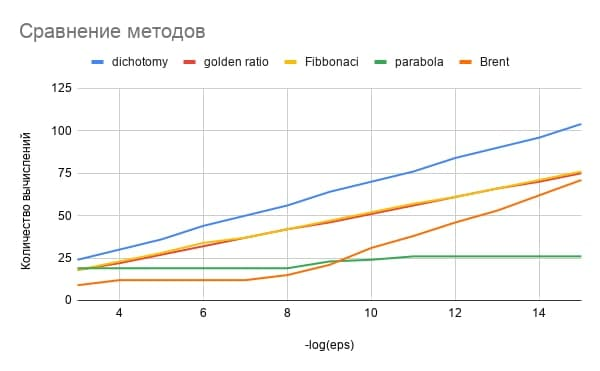
\includegraphics[width=1\textwidth]{new_methods.png}
\end{figure}

%\newpage
%\section{Работа алгоритмов на многомодальных функциях}

%\newpage
%\section{Выводы}

\end{document}